% !TEX root = ../main.tex
% Chapter Background information and theory

\chapter{State-of-the-art of conversational agents systems} % Main chapter title
% \chapter{Background information and theory} % Main chapter title

\label{Chapter2} % Change X to a consecutive number; for referencing this chapter elsewhere, use \ref{ChapterX}

A conversational agent (chatbot) is intended to respond to a Human by taking advantage of all its knowledge, its capacity to detect sentiments or remember the context, or its ability to search information on the web. Chatbots tend to use text as input and output format but it is also possible to use speech recognition and speech generation to allow users to speak.

\section{Different approaches to build a conversation agent}
Chatbots are created using two different approaches, namely the \textbf{Rule-based} approach and the \textbf{Generative} approach. The Rule-based approach, as its name indicates, uses rules to understand user input and pick from a list of answers a possible on. Rule-based chatbots exist since 1966 with the developement of ELIZA chatbot in \citet{Weizenbaum:1966:ECP:365153.365168}. ELIZA's goal was to measure the psychological effects on Humans when they talk to a machine. Some of the test subjects found it really hard to believe that they were talking to a computer. ELIZA follows a script and analyzes user input to find keywords and to choose the proper answer. The workload for the developper is quite intensive and it only takes one wrong answer that the developer might not have thought of and the user understands he is not talking to a Human.

The Generative approach is a machine learning model that takes advantage of the recent research and technology improvements enabling deep neural networks model to be trained on large datasets. The main difference with the rule-based approach is that the chatbot learns and establishes its own rules based on the training dataset. Thus, generative models are less entitled to misunderstand the user but since they learn themselves the output sentences, they might generate sentences with punctuation errors, grammatical errors, or even generate incomprehensible sentences. Aside the generation problems, training deep neural networks is not an easy task and require high performance hardware.

These two approaches are used in two different cases, closed-domain and open-domain conversations. The closed-domain conversation means that the chatbot can answers to a particular type of questions. For example, if a company develops a chatbot to let users manage their booking details, it will only be able to answer requests about bookings and nothing else. At contrary, an open-domain chatbot is able to discuss about anything. For example, Siri the personnal assistant developed by Apple or Alexa the personnal assistant developed by Amazon are able to understand very different requests and they are not blocking the user. Figure \ref{fig:types_chatbot} shows the different types of chatbots and hightlights the fact that the rule-based approach is only meant for closed-domain conversations. An open domain chatbot based on prepared scenarios and answered and following rules is impossible due to the amount of work needed to construct such a system.

\begin{figure}
    \centering
    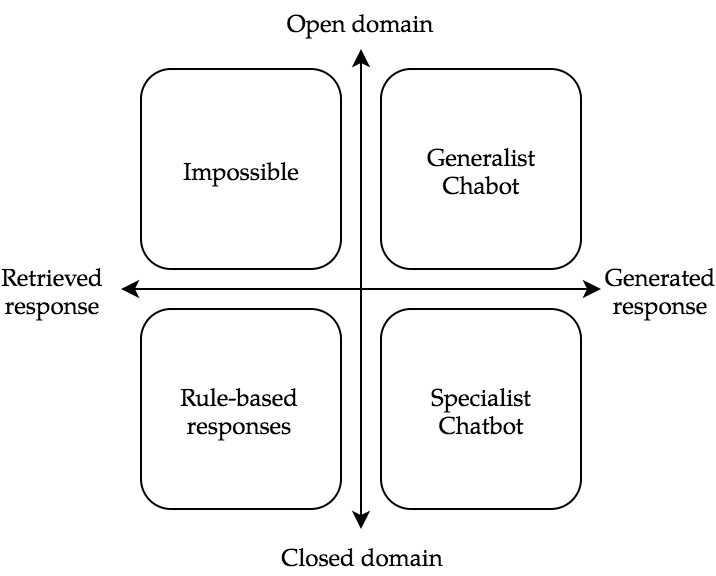
\includegraphics[width=.66\textwidth]{types_chatbot}
    \caption{Different types of chatbot}
    \label{fig:types_chatbot}
\end{figure}

\section{Rules-based models}
In this section, two technics to build a rule-based are presented, one emerged 16 years ago and the other 1 year ago.

\subsection{Artificial Intelligence Markup Language}
http://www.alicebot.org/aiml.html

\subsection{Development tools for rule-based conversational agents}
The interest around chatbots has risen the past year and half, as shows Figure~\ref{fig:trend_chatbot}. Different products appeared since then on the market to help businesses and privates build and deploy chatbots. One example is Dialogflow\footnote{\url{https://dialogflow.com/}} but most of the tools follow the same logic. The goal of Dialogflow is to understand the intent of the user and trigger an action. The action can be a text response provided by Dialogflow or, Dialogflow can use a webhook and send the intents to a remote server to build the response accordingly to user's intents.
For example, a possible application would be a chatbot that tells the student where is the next lecture. Dialogflow understands the intent and forwards the request to the webhook. The webhook receives the intent and connects to the school servers to get the information and send it back to the user. Figure~\ref{fig:dialogflow} shows the flow of interactions for a chatbot developed on Dialogflow.

\begin{figure}
    \centering
    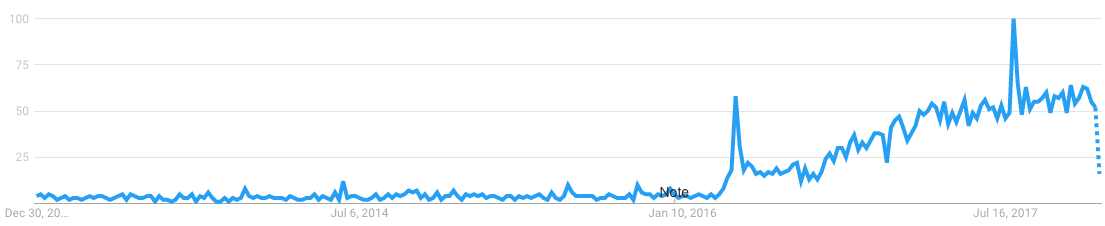
\includegraphics[width=\textwidth]{trend_chatbots}
    \caption[Web search interest for ``chatbot'']{Interest of the keyword ``chatbot'' in web searches for the past 5 years. Source: Google Trends}
    \label{fig:trend_chatbot}
\end{figure}

\begin{figure}
    \centering
    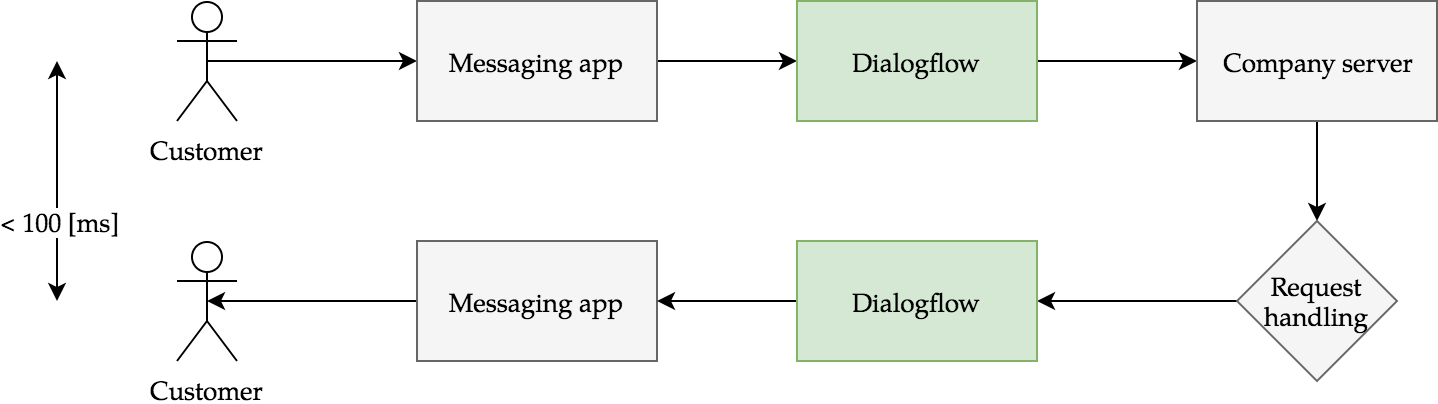
\includegraphics[width=\textwidth]{dialogflow_flow}
    \caption[Dialogflow based chatbot]{Flow of interactions for a chatbot developed on Dialogflow}
    \label{fig:dialogflow}
\end{figure}

The strength of these tools is that they extract the intent of the user without being restricted to an exact sentence. These tools are sometimes called hybrid because they are in their core rule-based models, but use Natural Language Processing to understand better the user. Thus, the chatbots are more reliable and therefore, more interesting for companies like Swiss, Comcast, The Wall Street Journal or Mecedes-Benz. However, the downside is that these chatbots are deployed over popular messaging platforms like Facebook Messenger or WhatsApp. Thus, the privacy of the data is questionable. For example, would Facebook use the information emitted from the Swiss arline chatbot to target ads for travelers?

\section{Generative approach}
Generative conversation models are based on a learning process and need a large set of training data (e.g. \citet{1506.05869} used 62M sentences). Generative models are created using deep neural networks like Recurent Neural Network (RNN) \citep{1503.02364,1506.05869}.

\subsection{Vector representation of words}

As RNNs take real vectors as inputs, the text sequence are represented as continuous vectors, known as word embeddings. A technic called word2vec \citep{1301.3781} proposes two log-linear models based on Feedforward Neural Net language Model (NNLM) to represent efficiently words in vector space. The first model architecture of word2vec is called the Continuous Bag-of-Words (CBOW) model and follow the feedforward NNLM architecture with one hidden layer. The idea behind is that we train a model to predict a word from a sentence using N (N$\in \mathtt{N}$) words occuring before and N words occuring after it in the sentence (e.g. in ``\textit{This corpus contains millions entities}'' and with N$=2$, the input's model are \textit{This, corpus, millions entities} and the target is \textit{contains}). Figure~\ref{fig:cbow} shows the CBOW architecture. The skip-gram architecture, represented in Figure~\ref{fig:skipgram}, takes as input the current word to predict the context. Empirical results \citep{tf.word2vec} show that the Skip-gram model is more useful for large datasets as for CBOW, it fits better on small datasets.

\begin{figure}
    \centering
    \begin{subfigure}{.45\textwidth}
        \centering
        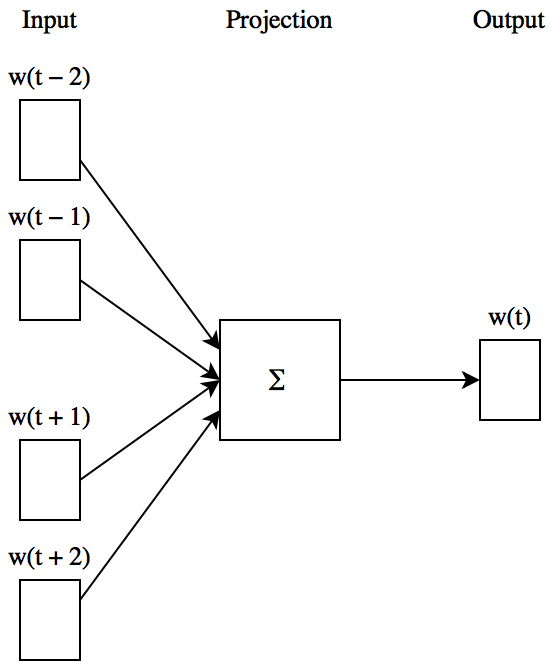
\includegraphics[width=.8\textwidth]{word2vec_cbow}
        \caption[Continuous Bag-of-Words architecture]{CBOW architecture from word2vec models. Context is used to predict the current word.}
        \label{fig:cbow}
    \end{subfigure}
    ~
    \begin{subfigure}{.45\textwidth}
        \centering
        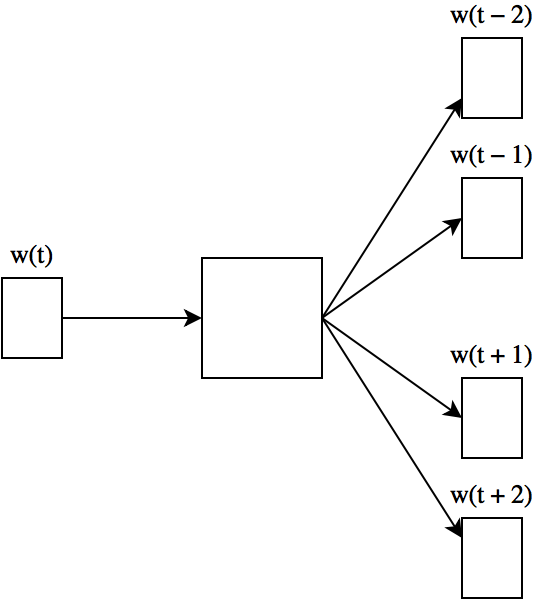
\includegraphics[width=.8\textwidth]{word2vec_skipgram}
        \caption[Skip-gram architecture]{Skip-gram architecture from word2vec models. Current word is used to predict the context.}
        \label{fig:skipgram}
    \end{subfigure}
    \caption{Word2vec architectures. Source:~\citet{1301.3781}}
    \label{fig:word2vec}
\end{figure}

An interesting finding by \citet{1301.3781} shows that simple arithmetic operations can be performed on word embeddings to highlight and find words sharing the same relation. For example, $\mathrm{queen} - \mathrm{king} + \mathrm{man} = \mathrm{woman}$.

\subsection{Recurrent Neural Networks}
Recurrent Neural Network (RNN) is a neural network created to analyze time-series. Given a sequence $\bm{x} = (x_1, ..., x_T)$, a RNN computes the hidden state $\bm{h} = (h_1, ..., h_T)$ and outputs the sequence $\bm{y} = (y_1, ..., y_T)$, iterating from time $t = 1$ to $T$.

\begin{align}
    \bm{h}_t &=
    \label{eq:rnn_h}
    \bm{y}_t &=
    \label{eq:rnn_y}
\end{align}

Vanilla RNNs present two main problems, described in~\citet{bengio1994learning}.
Bengio et al. (1994) detail vanishing and exploding gradient problems of RNN

1211.5063 answers exploding gradient problem with gradient clipping

Long short-term memory (LSTM) \citep{hochreiter1997lstm} is a RNN model having the capability of memorizing long distance information and being less affected by the vanishing gradient problem described in \citet{pascanu2013difficulty}. Instead of having a single activation function, for example $\tanh$, the LSTM cell has different gates interconnected with different functions. The following LSTM architecture is presented in \citet{1303.5778}.

\begin{align}
    \label{eq:lstm-cells_i}
    \bm{i}_t &= \sigma (\mathbf{W}_{xi}^{T} \cdot \bm{x}_t + \mathbf{W}_{hi}^{T} \cdot \bm{h}_{t-1} + \bm{b}_i)\\
    \label{eq:lstm-cells_f}
    \bm{f}_t &= \sigma (\mathbf{W}_{xf}^{T} \cdot \bm{x}_t + \mathbf{W}_{hf}^{T} \cdot \bm{h}_{t-1} + \bm{b}_f)\\
    \label{eq:lstm-cells_o}
    \bm{o}_t &= \sigma (\mathbf{W}_{xo}^{T} \cdot \bm{x}_t + \mathbf{W}_{ho}^{T} \cdot \bm{h}_{t-1} + \bm{b}_o)\\
    \label{eq:lstm-cells_g}
    \bm{g}_t &= \tanh (\mathbf{W}_{xg}^{T} \cdot \bm{x}_t + \mathbf{W}_{hg}^{T} \cdot \bm{h}_{t-1} + \bm{b}_g)\\
    \label{eq:lstm-cells_c}
    \bm{c}_t &= \bm{f}_t \odot \bm{c}_{t-1} + \bm{i}_t \odot \bm{g}_t\\
    \label{eq:lstm-cells_y}
    \bm{y}_t &= \bm{h}_t = \bm{o}_t \odot \tanh ( \bm{c}_t )
\end{align}

number \ref{eq:lstm-cells_o} is the output gate, \ref{eq:lstm-cells_i} is the input gate

\textbf{bidirectional LSTM, residual connections, dropout}
1409.2329 shows that dropout (UofT, srivastava, 2013) does not work well with RNNs. Moreover, people tend to use small RNNs models because large one tend to overfit. 1409.2329 answers these problems by applying dropout to a certain subset of the RNNs' connections (blabla how they used dropout differently on RNN and LSTM)

\subsection{Neural Machine Translation}
The Neurel Machine Translation (NMT) model, proposed by~\citet{nmt-phd},

The NMT model is inspired from the seq2seq architecture. Sequence-to-sequence (Seq2Seq) was first introduced by Google \citep{1409.3215} to be an end-to-end approach that makes only minimal assumptions on the sequence structure. Researchers observed that building end-to-end deep learning systems based on discriminative neural networks often work better with data minimally preprocessed~\citep{chen2015handbook}.  Among others, a notable difference is the input of the decoder. In Figure~\ref{fig:seq2seqmodel} that shows the seq2seq model architecture, the decoder's output $h_{t-1}$ is the decoder's input $x_{t}$. In the NMT model, the decoder is fed with target output embeddings.


\begin{figure}
    \centering
    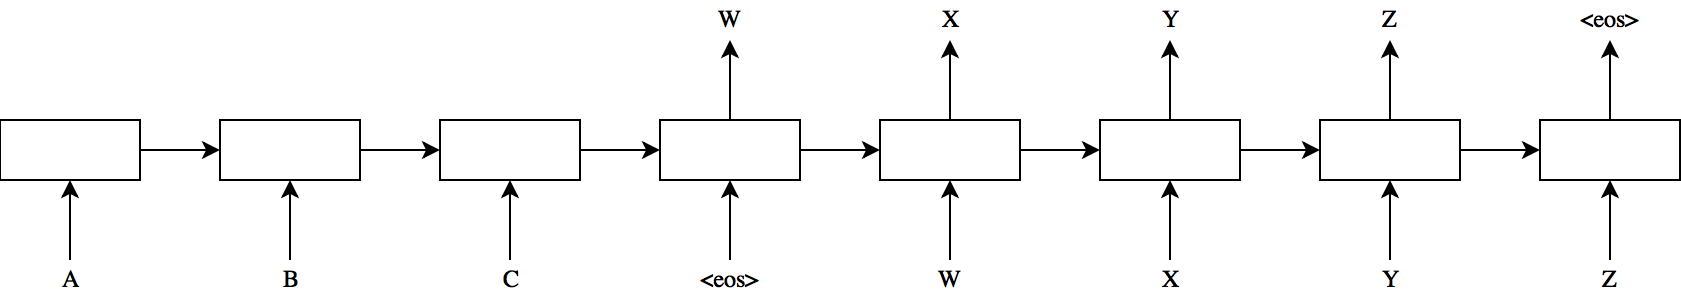
\includegraphics[width=\textwidth]{seq2seq_model}
    \caption[Seq2Seq model architecture]{Seq2Seq model architecture~\citep{1409.3215}. In the decoder part of the model, the output $h_{t-1}$ is the input $x_{t}$}
    \label{fig:seq2seqmodel}
\end{figure}

In the use case of chatbots, the input and output sequences, or conversations, can have basically any length, only be tokenized, and the NN is able to learn. Seq2Seq approach decompose the architecture in two main parts, namely the encoder and the decoder. The encoder takes as input a sequence of text and forms a fixed-size vector representation of it. The decoder uses this abstract representation produced by the encoder to output the adequate output sentence. The fixed-size vector representation is meant at capturing relevant information from the input sentence. Figure~\ref{fig:nmt} presents the workflow of a NMT model. The example shown is a translation problem, but NMT model architecture is used also for conversational agents or text summarization \citep{tensorflow.nmt}.

\begin{figure}
    \centering
    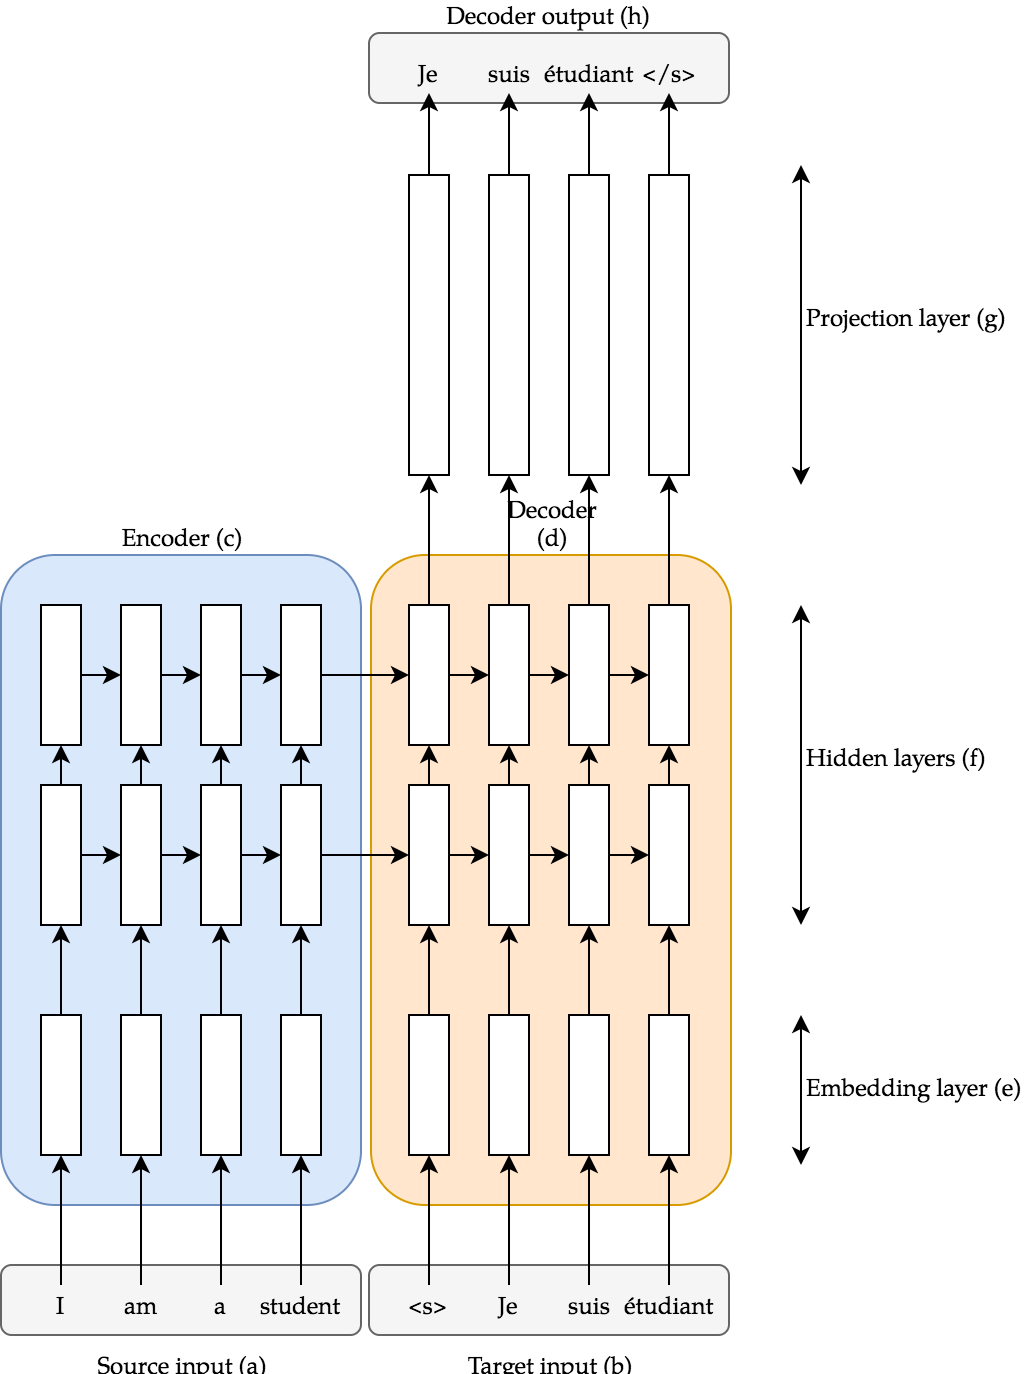
\includegraphics[width=.8\textwidth]{nmt_training_scheme}
    \caption[Neural Machine Translation model scheme]{Neural Machine Translation model \citep{tensorflow.nmt}. \textbf{(a)} \textit{Source input} refers to the input sequence tokenized to let the encoder read it token by token. \textbf{(b)} \textit{Target input} refers to the decoder input that let the decoder have the correct $t-1$ token and decode properly. \textbf{(c)} \textit{Encoder} refers to stacked RNN model used to build an abstract representation of the input sequence. \textbf{(d)} \textit{Decoder} refers to stacked LSTM that produce the output sequence based on the abstract representation built by the encoder and on the ``previous'' target word. \textbf{(e)} \textit{Embedding layer} refers to the feedforward neural network language model that creates words' vector representation. \textbf{(f)} \textit{Hidden layers} refers to the number of stacked RNN layers. \textbf{(g)} \textit{Projection layer} refers to the one-hot vector of the predicted word, used to calculate the loss. \textbf{(h)} \textit{Decoder output} refers to the output sequence tokenized.}
    \label{fig:nmt}
\end{figure}

Both the encoder and the decoder are RNN: LSTMs \citep{1409.3215,1508.04025} or GRUs \citep{1706.05125,1503.02364}. These RNN models take as input fixed-size sentences but conversations have varying length. To face this issue, the sentences are padded with $0$ vectors to reach the size of the longest sentence of the training set. However, a lot of computation and memory is required to save vectors filled with zeros and train a model. This computation leak is resolved by bucketing the training set based on the length of the sentence. With buckets, sentences are still zero padded to the longest sentence of the bucket but it ensures that the padding is minimized.

% \textbf{Calculate the number of parameters}

% \textbf{Evaluation: loss, perplexity, cross-entropy, BLEU, being an active research topic today}
The top-layer of the decoder is fed to a softmax function to produce the predictive distribution. This distribution is then used to extract the probability of every words being the target word or not, the most probable word is chosen and output. To know how good a model works, the cross-entropy is calculated between the target and decoded distribution and used as the loss function to backpropagate the error through the network.
Moreover, to measure how good model actually generates words, the BLEU score is used~\citep{bleu-score}. The BLEU score measures the closeness of words between the decoded and target sentences using a n-gram precision.
% \begin{equation}
%     \mathrm{BLEU} = XX, \mathrm{BLEU} \in [0, 100]
%     \label{equ:bleu}
% \end{equation}
In NMT, the BLEU score works well because a translation is often the same even with a different context. For example, ``maison'' in French will almost always be translated as ``house'' in English and until the word translation is not correct, the BLEU score is low and it makes sense.
However, when dealing with conversational agents, the context can vary a lot, from the way the user write to, for example, the weather (in the case the chatbot talks about weather). From this observation, \citet{1603.08023} showed that there are not currently a reliable method to measure the effectiveness of a chatbot, except the use of Human evaluators.

Once the model is trained, there are mainly two approaches to decode a sentence, known as inference, namely the greedy search or the beam search. The greedy search takes the most probable output word at each timestep and fed it in the decoder's input at $t+1$. This approach is computationnaly efficient but does not yield great quality. Figure~\ref{fig:nmt-inference} shows the inference process using a greedy search.
\begin{figure}
    \centering
    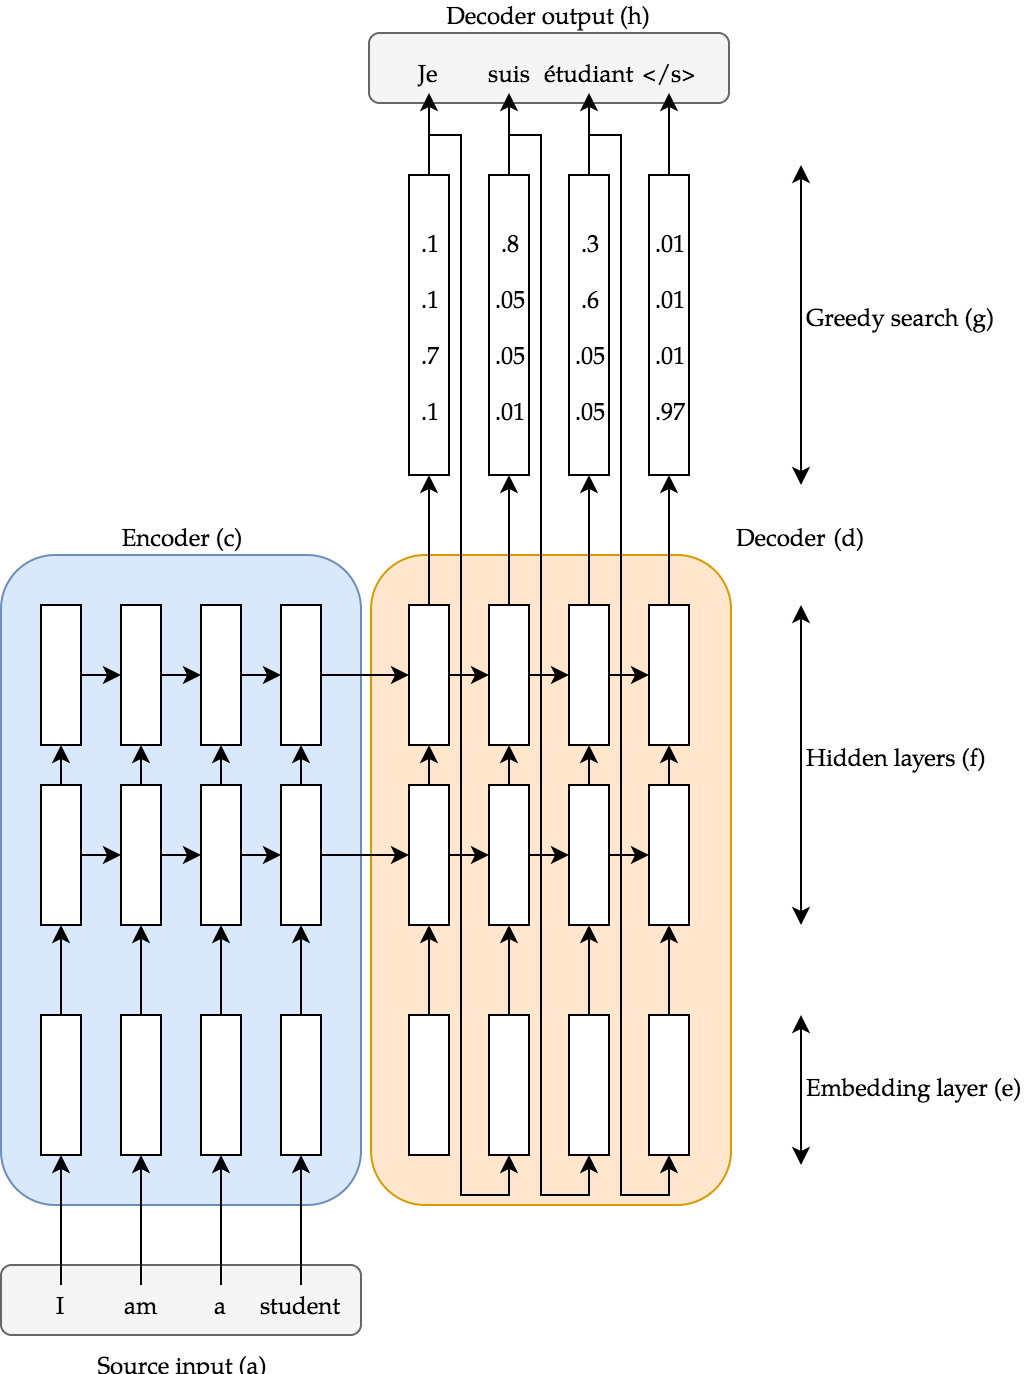
\includegraphics[width=.8\textwidth]{nmt_inference_scheme}
    \caption[Neural Machine Translation inference scheme]{Neural Machine Translation inference scheme \citep{tensorflow.nmt}. \textbf{(a)} \textit{Source input} refers to the input sequence tokenized to let the encoder read it token by token. \textbf{(b)} \textit{Target input} refers to the decoder input that let the decoder have the correct $t-1$ token and decode properly. \textbf{(c)} \textit{Encoder} refers to stacked RNN model used to build an abstract representation of the input sequence. \textbf{(d)} \textit{Decoder} refers to stacked LSTM that produce the output sequence based on the abstract representation built by the encoder and on the ``previous'' target word. \textbf{(e)} \textit{Embedding layer} refers to the feedforward neural network language model that creates words' vector representation. \textbf{(f)} \textit{Hidden layers} refers to the number of stacked RNN layers. \textbf{(g)} \textit{Projection layer} refers to the one-hot vector of the predicted word, used to calculate the loss. \textbf{(h)} \textit{Decoder output} refers to the output sequence tokenized.}
    \label{fig:nmt-inference}
\end{figure}

The beam search is computationnaly more expensive than the greedy search but yields much better quality. The process of the beam search is to keep track of the most probable words at each time step and to feed the decoder's input with the N most probable words until the number of possibilities excess a certain threshold. At each time, the probabily of the whole sequence is calculated and only the words being in the most probable sentence are kept for $t+1$.


\subsection{Attention mechanism}
Intuitively, when one translates a sentence, one does not only read the sentence once and straightly translates it. The translation is based on the sentence overall and the translator goes back and forth in the source sentence to give the proper translation. The same intuition applies in conversations.
In basic seq2seq architecture, the model only bases its input data knowledge on the encoder's last hidden state. \citet{1508.04025} proposed a simpler method to allow the model to pay attention to what matters at every timestep, based on the research conducted by \citet{1409.0473} that proposed an improvement in seq2seq model performance by allowing ``\textit{the model to automatically (soft)-search for parts of a source sentence that are relevant to predicting a target word}''.

\begin{figure}
    \centering
    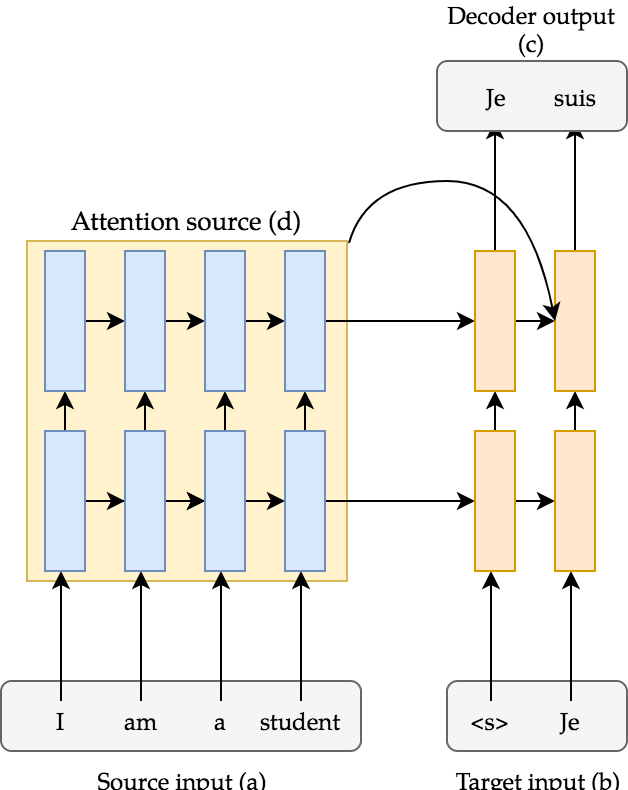
\includegraphics[width=.6\textwidth]{attention_basic_scheme}
    \caption[Attention basic scheme]{Attention basic scheme. The decoder uses what is relevant from the input source to decode the sentence and not only the last hidden state of the encoder. Source:~\citet{youtube-nmt-attention}}
    \label{fig:attention_basic_scheme}
\end{figure}

The attention mechanism can be seen as a memory which the model retrieves information when needed. Figure~\ref{fig:attention_basic_scheme} shows the decoder taking into account attention in the decoding process. \citet{1508.04025} proposed a simple and effective approach of the attention mechanism separated into two models, namely the \textit{global attention} and \textit{local attention}, following nevertheless a common ground. At each time step $t$, the hidden-state $\bm{h}_t$ at the top layer of the stacked LSTMs is taken to construct a context vector $\bm{c}_t$.
The context vector $\bm{c}_t$ captures relevant source-side information that helps predicting the current target word $\bm{y}_t$. As for the basic NMT model, the decoder output is sent to a softmax function to output the predictive distribution. In an attention-based NMT, the current hidden state $\bm{h}_t$ is concatenated with the context vector $\bm{c}_t$ to produce an attentional hidden state, as showed in Equation~\ref{equ:atn-hidden-state}, whose fed through the softmax layer, as showed in Equation~\ref{equ:atn-hidden-state-to-softmax}.
\begin{equation}
    \bm{\tilde{h}}_t = \tanh ( \mathbf{W}_c [\bm{c}_t;\bm{h}_t])
    \label{equ:atn-hidden-state}
\end{equation}
\begin{equation}
    p( y_t | y _{<t}, x) = \mathrm{softmax(\mathbf{W_s}\bm{\tilde{h}_t})}
    \label{equ:atn-hidden-state-to-softmax}
\end{equation}
 The global and local attention models differ on how the context vector $\bm{c}_t$ is derived.

 The global attentional model takes into account all the hidden states of the decoder to produce the context vector $\bm{c}_t$. This model compares the current target hidden $\bm{h}_t$ with each source hidden state $\bm{\bar{h}}_s$ to derive a variable-length alignment vector $\bm{a}_t$ whose size equals the number of time steps on the source side.
 \begin{align}
    \bm{a}_t(s) &= \mathrm{align}(\bm{h}_t, \bm{\bar{h}}_s)\\
    \label{equ:atn-a_t}
    &= \frac{\mathrm{exp}(\mathrm{score}(\bm{h}_t, \bm{\bar{h}}_s))}{\sum_{s'} \mathrm{exp}(\mathrm{score}(\bm{h}_t, \bm{\bar{h}}_{s'}))}
 \end{align}
The score function $\mathrm{score}(\bm{h}_t, \bm{\bar{h}}_s)$ is presented in three different alternatives in~\citet{1508.04025}, as described in Equation~\ref{equ:atn-score}.
\begin{subequations}
    \label{equ:atn-score}
    \begin{align}[left ={\mathrm{score}(\bm{h}_t, \bm{\bar{h}}_s) = \empheqlbrace}]
        & \bm{h}_t^T \bm{\bar{h}}_s & \mathit{dot} \label{equ:atn-score-dot}\\
        & \bm{h}_t^T \mathbf{W_a} \bm{\bar{h}}_s & \mathit{general} \label{equ:atn-score-general}\\
        & \bm{v}_a^T \tanh ( \mathbf{W_a} [\bm{h_t}^T;\bm{\bar{h}}_s]) & \mathit{concat} \label{equ:atn-score-concat}
    \end{align}
\end{subequations}
The first alternative of the score function is described in Equation~\ref{equ:atn-score-dot} and simply performs a dot product between the decoder hidden state and encoder hidden state and tries to find the words that are similar.
The score function described in Equation~\ref{equ:atn-score-general} resembles to the ``\textit{dot}'' score function but instead, places a weight matrix in-between to let the model capture what part of the hidden states are relevant. \citet{youtube-nmt-attention} highlights the \textit{``general''} approach as working better than the two others and being the form well-adpoted by the community.
The last alternative of the score function, described in Equation~\ref{equ:atn-score-concat}, is the one proposed by \citet{1409.0473}. In this situation, the score function is like a neural network layer and the decoder and encoder hidden states are concatenated together, then multiplied by a weight matrix, fed to a sigmoid function and finally multiplied by a vector. The main concern with the last alternative is that the two hidden states are not interacting with each other.
\citet{1508.04025} approach is similar to \citet{1409.0473} but they have three main differences that simplifies and generalizes the concept. First, in \citet{1409.0473}, instead of using only the top hidden states, the model concatenates all source hidden states of the bidirectional encoder to the target hidden states.
Secondly, \citet{1409.0473} computation path requires hidden states from previous time whereas in \citet{1508.04025}, only the current time hidden states are used. Finally, as mentionned before, \citet{1409.0473} used the third function score, described in Equation~\ref{equ:atn-score-concat}.
Figure~\ref{fig:atn_global} shows the global attention model.

\begin{figure}
    \centering
    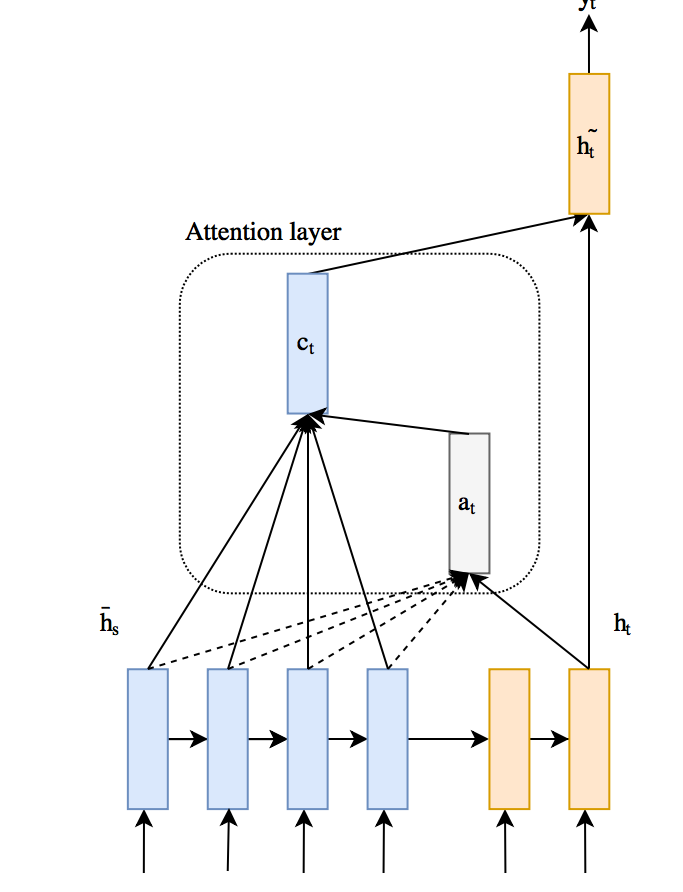
\includegraphics[width=.6\textwidth]{atn_global}
    \caption[Global attention model]{Global attention model. At each time step $t$, the model derives an alignment vector $\rm{a}_t$ by comparing the source hidden states $\rm{\bar{h}}_s$ and the current target state $\rm{h}_t$ with a score function.}
    \label{fig:atn_global}
\end{figure}

The local attentional model, proposed by \citet{1508.04025}, uses only a certain window around a position to compute the context vector. In other terms, it does not focus on everything at each timestep. In comparison to the global attentional model, the local attentional model is less expensive since it choses the subset of the source positions per target word. At each time step t, the context vector is created as a weighted average over the set of source hidden states within the window $[p_t - D, p_t + D]$, $D$ being empirically chosen.
This windows allows the attentional vector $\rm{a}_t$ to have a fixed size ($\rm{a}_t \in \mathbb{R}^{2D+1})$. The $p_t$ parameter can be set by methods. The \textit{monotonic alignment} simply sets $p_t = t$, assuming the source and the target sequences are somewhat aligned. The \textit{predictive alignment} learns and predicts $p_t$ in a form of a single layer feedforwoard neural network, as shows in Equation~\ref{equ:atn-pt-local-align}, $S$ being the sentence length.
\begin{equation}
    p_t = S \cdot \mathrm{sigmoid} ( \rm{v}_p^T \tanh ( \mathbf{W}_p \rm{h}_t))
    \label{equ:atn-pt-local-align}
\end{equation}
The position $p_t$ is taking into account to construct the alignment vector $\rm{a}_t(s)$ as defined in Equation~\ref{equ:atn-at-pt}, the standard deviation being empirically set as $\phi = \frac{D}{2}$.
\begin{equation}
    \rm{a}_t(s) = \mathrm{align}(\rm{h}_t, \rm{\bar{h}}_s) \mathrm{exp}(- \frac{(s - p_t)^2}{2\phi^2})
    \label{equ:atn-at-pt}
\end{equation}
Figure~\ref{fig:atn-local} shows the local attention model.
\begin{figure}
    \centering
    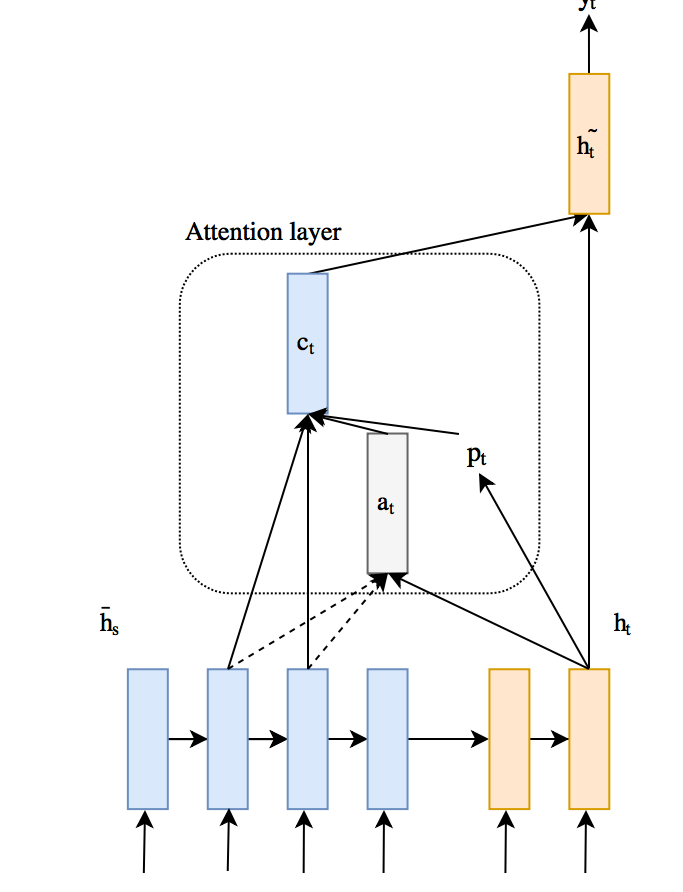
\includegraphics[width=.6\textwidth]{atn_local}
    \caption[Local attention model]{Local attention model. The alignment vector $\rm{a}_t$ is inferred from a selected window of hidden states $\rm{\bar{h}}_t$. The position $p_t$ is learned and predicted to have a better alignment between the source hidden states $\rm{\bar{h}}_s$ and the curret target state $\rm{h}_t$}
    \label{fig:atn-local}
\end{figure}

\section{Advanced conversational agents}
Despite the fact that NMT can be used as an architecture for chatbots, more advanced models use other components that empower the chatbot with more capabilities like sentiment analysis or information retrieval.

\subsection{Emotional conversational agents}
Chatbots are interesting to discuss with and sometimes they are useful, but in certain domain, like psychology, being able to react sentimentaly according to user's feelings can improve user experience and accomplish the awaited result. \citet{ecm-1704.01074} proposed an ``\textit{end-to-end framework to incorporate emotion influence in large-scale conversation generation}'' called the Emotional Chatting Machine (ECM). The model baseline is the same as the NMT model augmented with the attention mechanism, but ECM incorporates in addition to that two memory layers, an internal and an external memory.  


\subsection{Amazon Alexa}
Present the paper and how does a model for Alexa works? => Dialogue manager with submodels that takes care of ONE job and the dialogue manager calculates the probability for the submodels to really answer the question. Submodels also provide a confidence score to help the dialogue manager?
